

\section{Data Analysis}
\label{sec:dataAnalysis}


\subsection{Basic parameters of the deployed WR-based system}

\attention{The analyzed data consists of two sets of 2706160 \mbox{timestamps} collected over an undisturbed
system run of 31~days, 7~hours, 42~minutes and 40~seconds (Fri, 18 May 2012 22:38:53 GMT to 
Tue, 19 Jun 2012 06:21:33 GMT). The data was logged by the two SPECs (\textit{local} 
and \textit{loopback}) which used Fine Delay modules for timestamping the PPS reference signal 
(\figurename~\ref{fig:wrLNGStiming}).}
An extract from the timestamp logs is presented in Table~\ref{tab:rawData}. A visual inspection of the raw data 
shows a constant offset with respect to the reference PPS edge which occurs at \attention{0 nanoseconds}. 
This offset can be attributed to the different lengths of the cables connecting 
the reference PPS outputs to the inputs of the SPECs and that of the grandmaster switch as well as 
the internal delays of the switch locking to the reference PPS and the 10~MHz clock. 

% Importantly, the offset is the same for timestamps from both SPECs (\textit{local and loopack}) to within 
% instability which is the subject of further analysis.

The values of the Time Error (TE) were derived from the raw data by calculating the difference 
between a timestamp and an ideal PPS (occurring at \attention{0 nanoseconds}) and removing the average offset. 
The TEs for the \textit{local} and \textit{loopback} SPEC measurements are denoted $x_{lo}$ 
and $x_{lb}$ respectively (Table~\ref{tab:notRawData}). The performance of the system 
(two switches, two fiber links of 8.3~km each and two SPECs) can be characterized by calculating the 
difference (TE) between the corresponding timestamps from both SPECs, denoted $x_{diff}$ 
(Table~\ref{tab:notRawData}). The value of $x_{diff}$ with the average offset removed is \modified{denoted} 
$x_{diff-offset}$. 

% The TE values ($x_{lo}$, $x_{lb}$, $x_{diff}$ and $x_{diff-offset}$) 
% are used in this analysis to derived parameters of the deployed system. 

\begin{table}[!t]
\caption{Analyzed timestamps -- raw data}
\centering
\begin{tabular}{| l | c| c | c | c |}          \hline
& \multicolumn{2}{|c|}{\textbf{Local PPS }}  &  
\multicolumn{2}{|c|}{\textbf{Loopback PPS}}   \\   \hline
& \textbf{UTC} & \textbf{nanoseconds} & \textbf{UTC} & \textbf{nanoseconds} \\   \hline

1       & 1337380733 & 999999885.959 & 1337380733 & 999999885.500 \\   \hline
2       & 1337380734 & 999999886.014 & 1337380734 & 999999885.285 \\   \hline
3       & 1337380735 & 999999885.934 & 1337380735 & 999999885.338 \\   \hline
4       & 1337380736 & 999999885.906 & 1337380736 & 999999885.420 \\   \hline
...     &      ...   &  ..           &     ..     &      ..       \\   \hline
2706160 & 1340086893 & 999999885.879 & 1340086893 & 999999885.258 \\   \hline
         
\end{tabular}
\label{tab:rawData}
\end{table}

%\begin{table}[!t]
%\caption{Analyzed timestamps -- raw data}
%\centering
%\begin{tabular}{| l | c| c | c | c |}          \hline
%& \multicolumn{2}{|c|}{\textbf{Local PPS }}  &  
%\multicolumn{2}{|c|}{\textbf{Loopback PPS}}   \\   \hline
%& \textbf{UTC} & \textbf{nanoseconds} & \textbf{UTC} & \textbf{nanoseconds} \\   \hline
%
%1    & 1336823054 & 999999885.947266 &  1336823054 & 999999885.460938 \\   \hline
%2    & 1336823055 & 999999885.785156 &  1336823055 & 999999885.460938 \\   \hline
%3    & 1336823056 & 999999885.757812 &  1336823056 & 999999885.353516 \\   \hline
%4    & 1336823057 & 999999886.027344 &  1336823057 & 999999885.433594 \\   \hline
%...  &  ... & .. & .. & .. \\   \hline
%3719 & 1336826772 & 999999885.730469  & 1336826772 & 999999885.136719 \\   \hline
%\end{tabular}
%\label{tab:rawData}
%\end{table}


\begin{table}[!t]
\caption{Time Errors (TEs)}
\centering
\begin{tabular}{| l | c| c | c | c |}          \hline
& \textbf{$x_{lo}$} & \textbf{$x_{lb}$} & \textbf{$x_{diff}$} & \textbf{$x_{diff-offset}$}\\   \hline
       & [ns]  &  [ns]  & [ns]  &  [ns]  \\   \hline
1      & 0.043 & -0.015 & 0.459 & -0.058 \\   \hline
2      &-0.172 &  0.040 & 0.729 &  0.212 \\   \hline
3      &-0.119 & -0.040 & 0.596 &  0.079 \\   \hline
4      &-0.037 & -0.067 & 0.486 & -0.031 \\   \hline
...    &  ...  &  ...   &  ...  &  ...   \\   \hline
2706160&-0.037 & 0.0671 & 0.621 & 0.104 \\   \hline
\end{tabular}
\label{tab:notRawData}
\end{table}

\begin{figure}[!t]
\centering
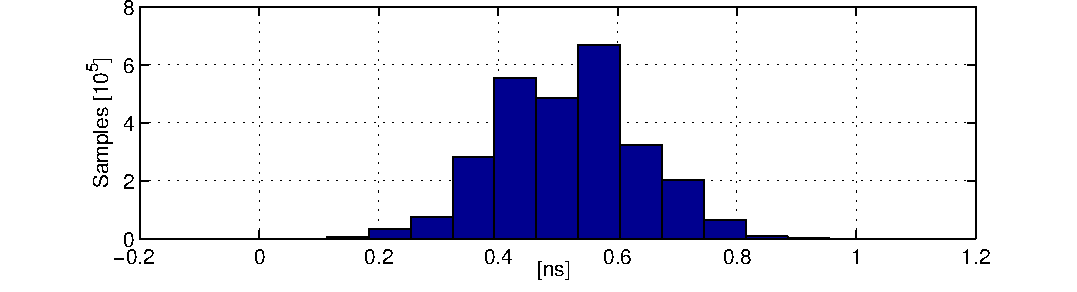
\includegraphics[width=0.5\textwidth]{../../figures/measurements/histogram-small.eps}
% \caption{A plot of the Time Error data with removed offset
% ($x_{lo}$, $x_{lb}$ and $x_{diff-offset}$) and a histogram of the difference between timestamps 
% acquired by the two SPECs ($x_{diff}$) which reflects system's performance.}
\caption{A histogram of the difference between timestamps 
acquired by the two SPECs ($x_{diff}$) which reflects system's performance.}
\label{fig:teAndHist}
\end{figure}


% \figurename~\ref{fig:teAndHist} presents a histogram of difference TE values ($x_{diff}$).
% Analysis of $x_{diff}$ are used to evaluate system accuracy and precision i.e. 

\figurename~\ref{fig:teAndHist} presents a histogram of $x_{diff}$ distribution. 
The average value of $x_{diff}$ marks the accuracy of the system and amounts to 0.517~ns
while the standard deviation of $x_{diff}$ reflects its precision which is 0.119~ns.
It is important to remember that these values include timestamping inaccuracy of the 
Fine Delay \cite{biblio:fineDelay} module (i.e. std. dev of 55~ps). 
% \attention{Therefore, 
% the numbers need to be understood as the characteristics of a complete system.}
The standard deviations calculated for $x_{lo}$ and $x_{lb}$ are 0.129~ns and 
0.125~ns respectively.

The Overlapping Allan Deviation calculated from the collected data is presented in 
\figurename~\ref{fig:oADEV}. The plot indicates White or Flicker PM Noise. 

\begin{figure}[!t]
\centering
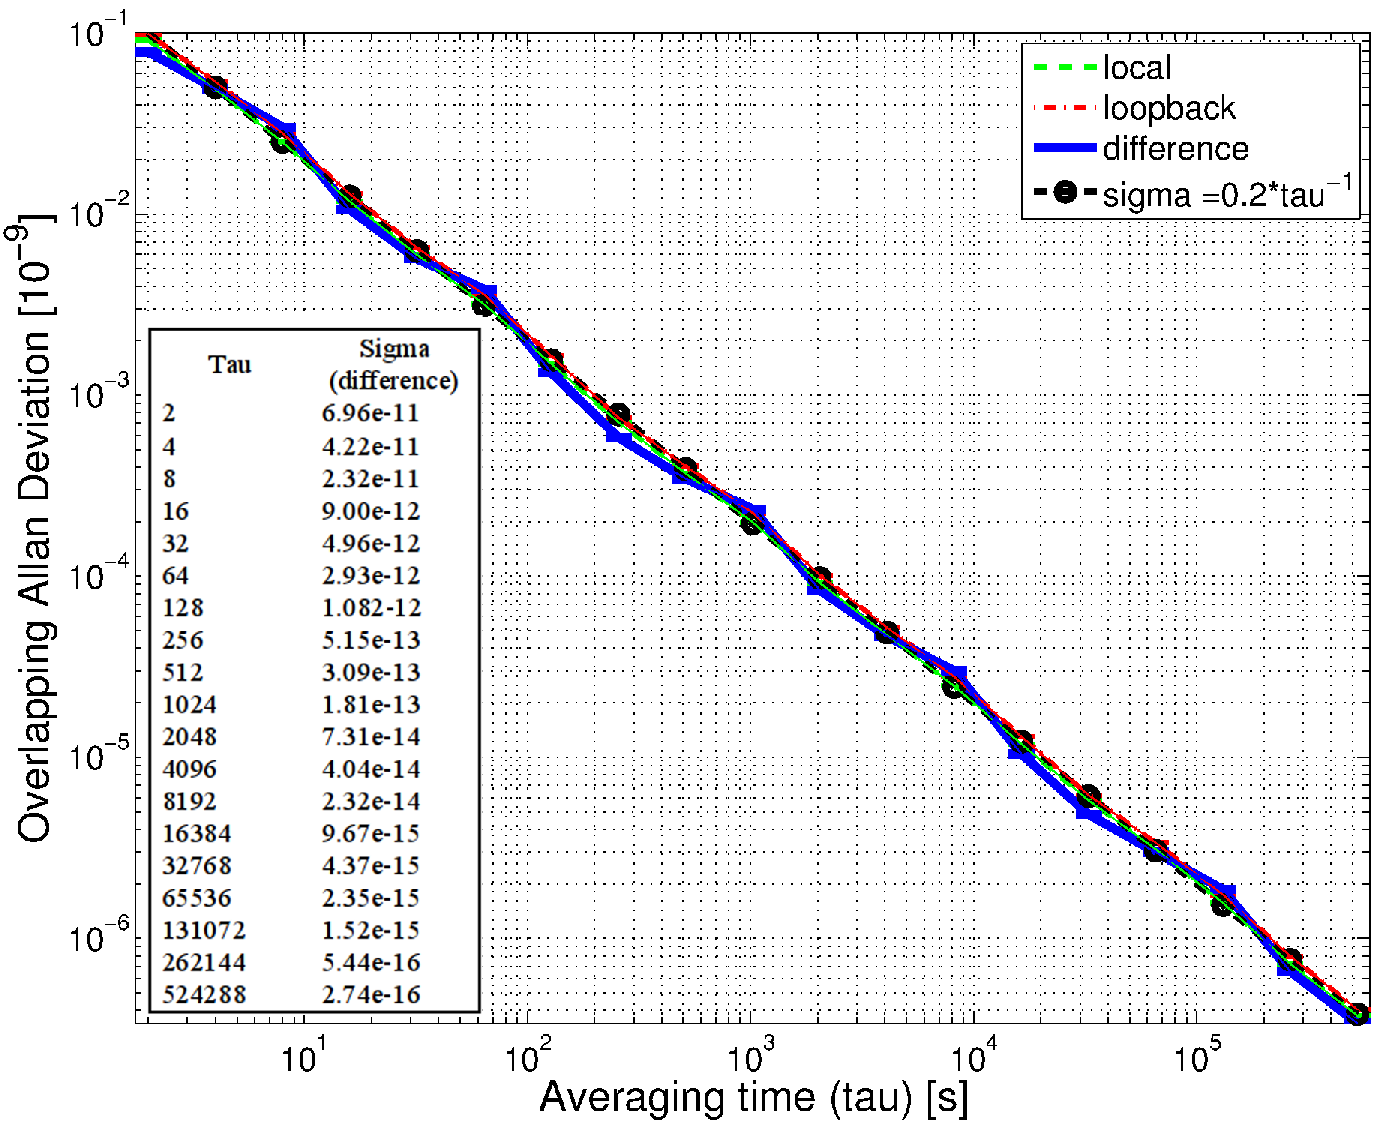
\includegraphics[width=0.4\textwidth]{../../figures/measurements/cngs_oADEV3.eps}
\caption{Overlapping Allan Deviation.}
\label{fig:oADEV}
\end{figure}

% The Maximum Time Interval Error (MTIE) presented in \figurename~\ref{fig:MTIE-no-cor} shows worse 
% performance of the \textit{local} SPEC compared to the \textit{loopback} SPEC. Removal of 9
% outliers from the \textit{local} SPEC data gives a more reasonable MTIE graph presented in
% \figurename~\ref{fig:MTIE-cor}. The cause of the outliers requires further investigation but it
% seems reasonable to suspect hardware or setup problem of the \textit{local} SPEC.  
% The Maximum Time Interval Error (MTIE) presented in \figurename~\ref{fig:MTIE-cor} proves the sub-nanosecond 
% performance of the system within the measurement period. The MTIE of $x_{diff}$ stabilizes at 
% around 0.95ns for the observation window values:
% \begin{equation}
%   \label{eq:mtie}
%   \approx 2048s (34min) < tau < 464074s (128.91h)
% \end{equation}
% 
% More data is highly desired to analyze a long term performance. 

The Maximum Time Interval Error (MTIE) of $x_{lo}$, $x_{lb}$ and $x_{diff-offset}$ 
was calculated for windows of $N_{tau}=2^k$ samples (k=1,2,3,...,21) and a window of the entire 
set of 2706160 samples. An optimized algorithm for MTIE
computation, called boundaries decision method \cite{biblio:MTIE}, was used to process 
\attention{the considerable number of samples in a reasonable time.}
The obtained MTIEs, depicted in \figurename~\ref{fig:MTIE},
indicate that the peak time deviations of the measured PPS signals (blue and green) are less than 1.15ns. 
However, the peak deviation between the two PPS measurements (blue) is smaller by 100ps 
(below 1.05~ns). It is important to mention that out of over 
2 millions measurements, only 9 values of $x_{diff-offset}$, 25 values of $x_{lo}$ and 146 values of 
$x_{lb}$ exceeded the $\pm$0.5~ns range. This constitutes 
0.0003$\%$, 0.0009$\%$ and 0.005$\%$ of the collected data respectively. The fact that the 
MTIE of $x_{diff-offset}$ is lower than the MTIEs of $x_{lo}$ and $x_{lb}$ might indicate 
external factor(s) affecting the entire system (thus removed with differential measurement) such
as temperature fluctuation.


\begin{figure}[!t]
\centering
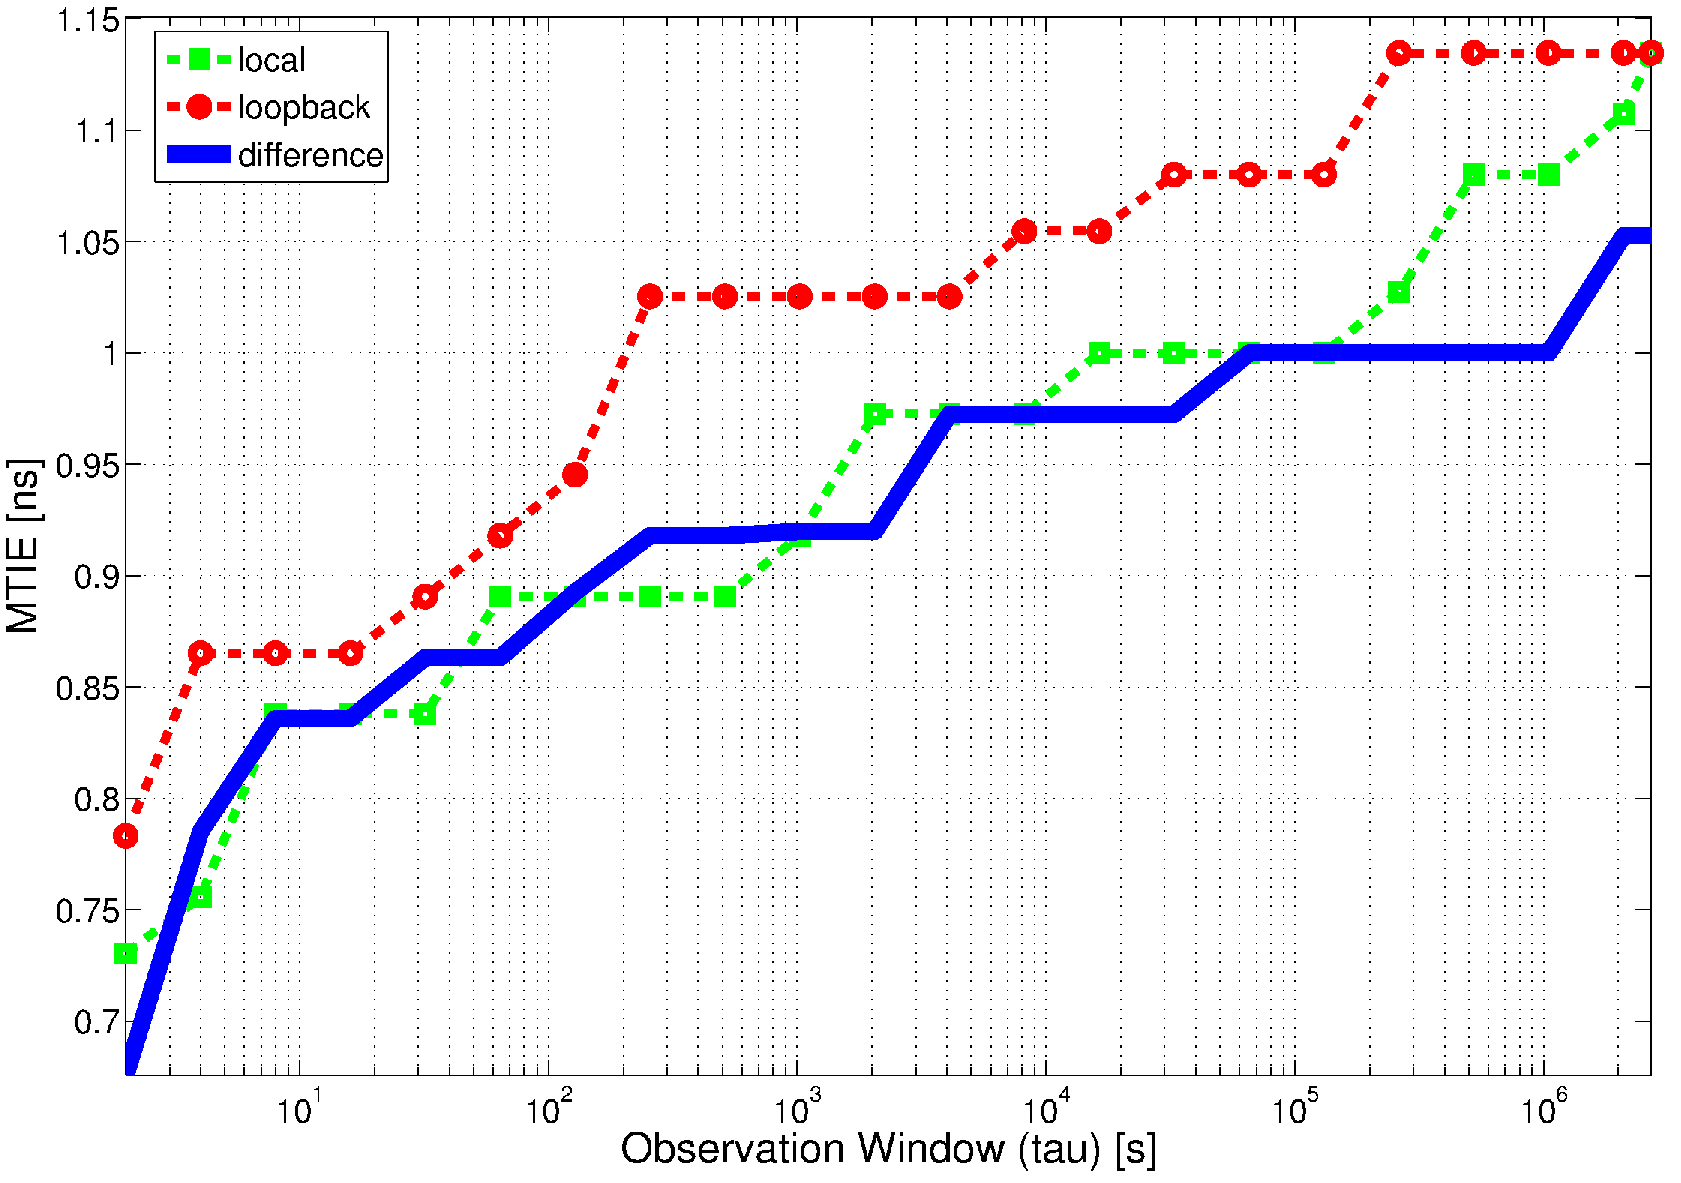
\includegraphics[width=0.4\textwidth]{../../figures/measurements/MTIE2.eps}
\caption{Maximum Time Interval Error (MTIE).}
\label{fig:MTIE}
\end{figure}

\subsection{Influence of temperature on the deployed WR-based system}

The temperature in the WR Room (\figurename~\ref{fig:wrLNGStiming}), where the grandmaster
switch and two monitoring SPECs are located, was logged over a substantial
part of the system run (Fri, 25 May 2012 14:00:00 GMT to Tue, 19 Jun 2012 06:00:00 GMT).
This temperature changed by 3.5 degrees Celsius over 25 days of observation time and 
a fraction of a degree on a daily basis, as depicted in \figurename~\ref{fig:temp.vs.TE} 
\modified{(upper plot)}. 
The blue sinusoid in the plots of \figurename~\ref{fig:temp.vs.TE} represents day-night cycles where the maximum indicates 
12:00 (local time) and minimum indicates 00:00 (local time). The lower plot of \figurename~\ref{fig:temp.vs.TE}
shows differential TE values ($x_{diff}$) which do not reveal noticeable changes with temperature. 

\begin{figure}[!t]
\centering
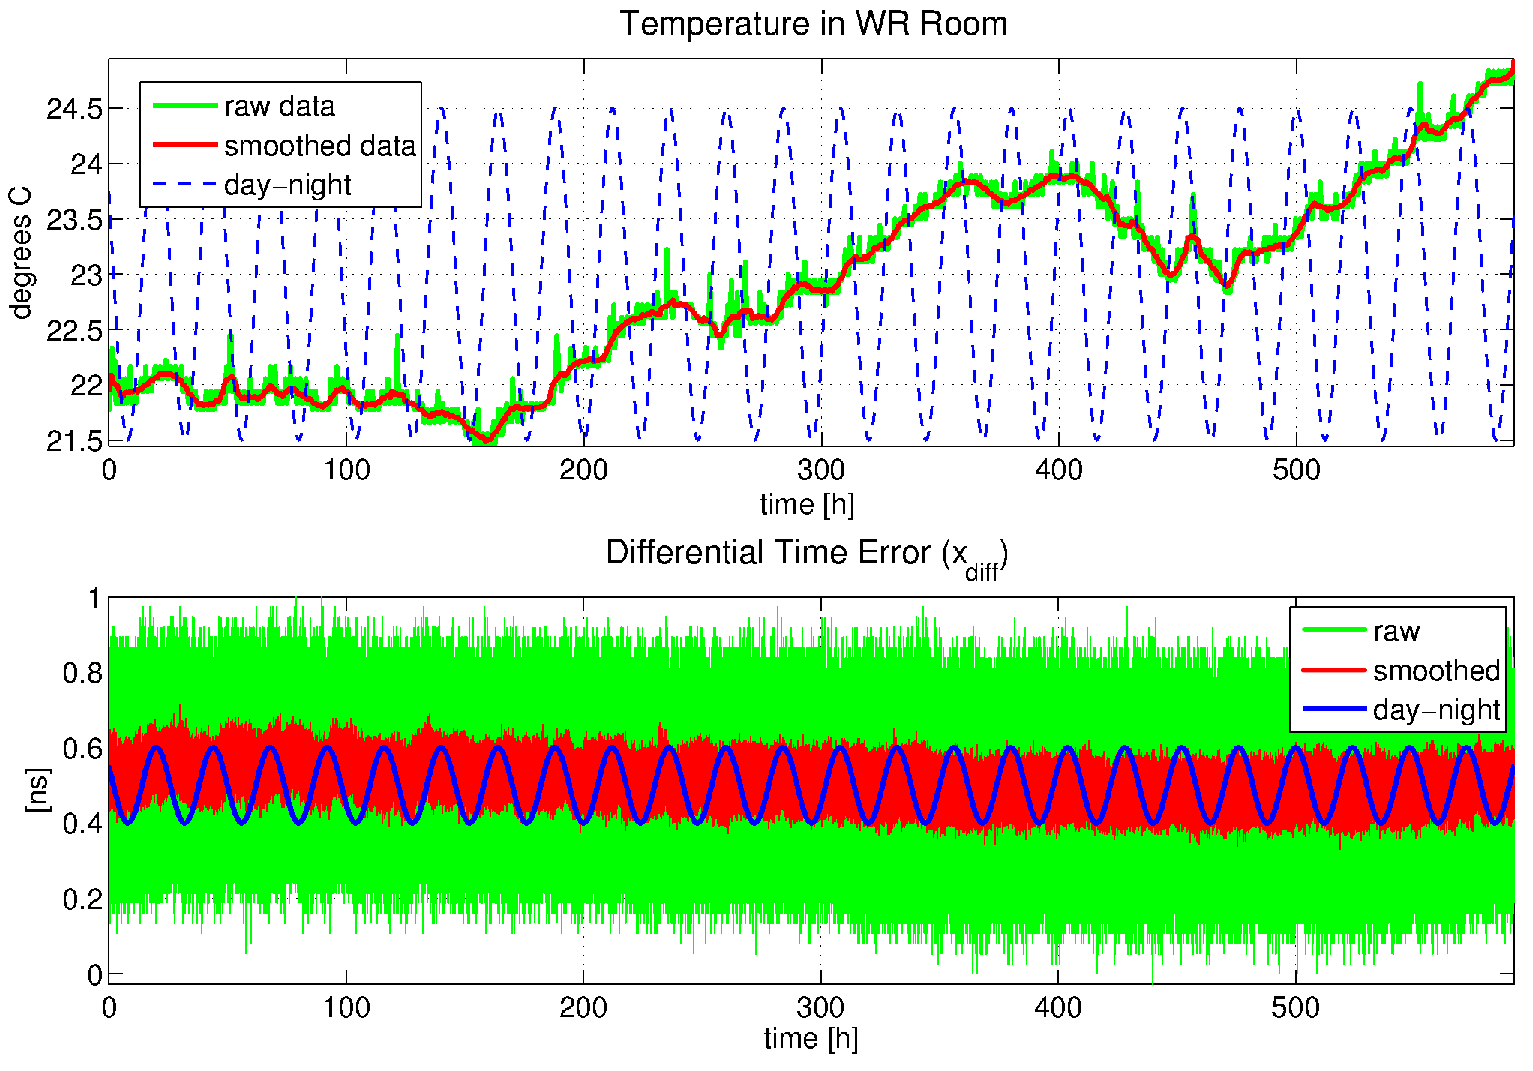
\includegraphics[width=0.4\textwidth]{../../figures/measurements/cngs_temp.vs.TE.eps}
\caption{Time Error versus temperature in WR Room.}
\label{fig:temp.vs.TE}
\end{figure}

Application of a 30 minutes-based averaging filter and smoothing of the raw data 
\modified{($x_{diff}$, $x_{lo}$ and $x_{lb}$)} enables to observe 
\modified{(\figurename~\ref{fig:temp.vs.filteredTE}, lower plot)}
a clear correlation between fluctuation of both SPECs' timestamps. The red line in 
\figurename~\ref{fig:temp.vs.filteredTE} (lower plot) shows fluctuation of timestamps measured by the 
\textit{local} SPEC \modified{($x_{lo}$)} while the blue line shows the fluctuation of the timestamps measured by the 
\textit{loopback} SPEC \modified{($x_{lb}$)}. Both lines
are correlated with a changing offset ($x_{diff}$) marked with the black line. For clarity,
WR Room temperature is depicted in the upper plot of the figure. The 
long-term oscillation of the differential TE ($x_{diff}$ in black) is not correlated 
with the temperature in the WR Room as the temperature keeps increasing while the 
$x_{diff}$ does not keep decreasing.
\figurename~\ref{fig:temp.vs.filteredTE} might indicate two sources of TE 
($x_{lo}$ and $x_{lb}$) fluctuation: (1) fluctuation of the entire WR-timebase with respect
to the reference PPS or (2) similar error introduced by the Fine Delay modules placed in the 
same location due to similar temperature variations.
The temperature monitored on the Fine Delay modules is stable to within 1 degree Celsius. Therefore,
\attention{the observed simultaneous fluctuation of both SPEC measurements} is most probably attributed to a factor not 
related with WR network (e.g. 10~MHz Fanout, \figurename~\ref{fig:wrLNGStiming}).

\begin{figure}[!t]
\centering
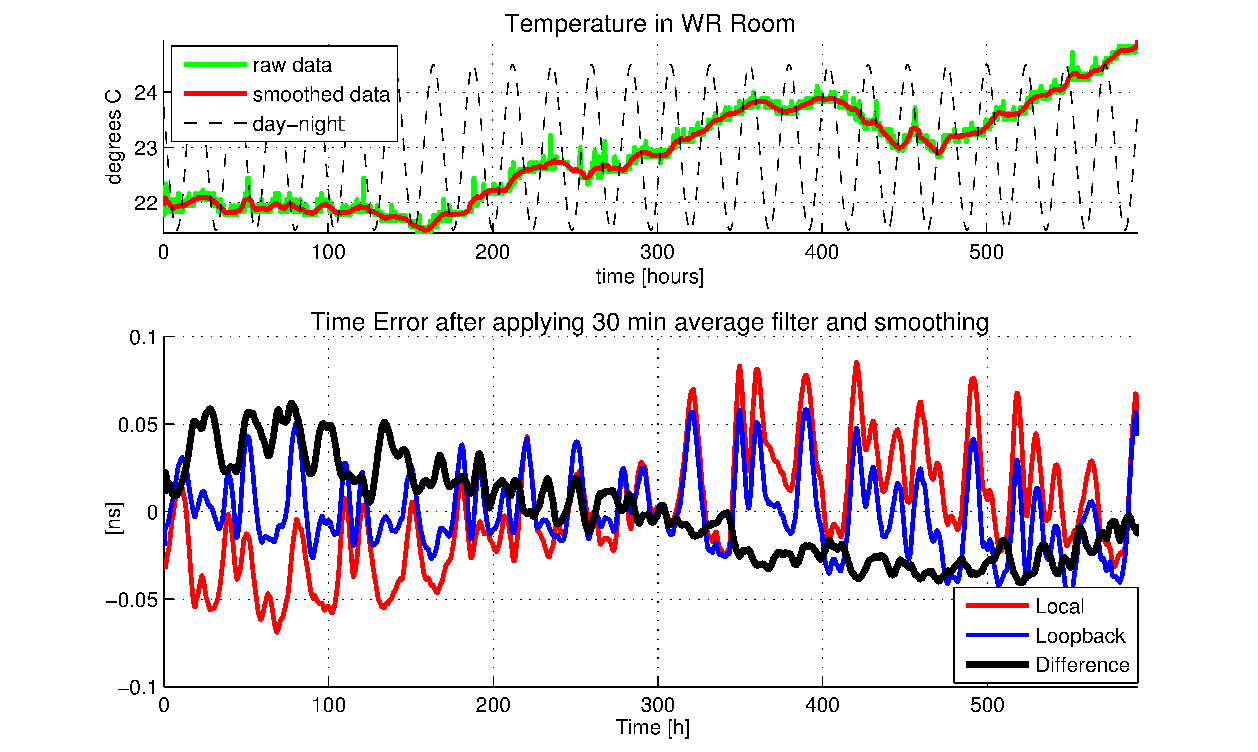
\includegraphics[width=0.5\textwidth]{../../figures/measurements/cngs_temp.vs.filteredTE3.eps}
\caption{Time Error (after applying 30 min average filter and smoothing) versus temperature in WR Room.}
\label{fig:temp.vs.filteredTE}
\end{figure}

% \begin{figure}[!t]
% \centering
% \includegraphics[width=0.5\textwidth]{newFig/temp.vs.FD.eps}
% \caption{Time Error versus temperature in WR Room and on the Fine Delay (~23 July 20 to ~11:30 July 22).}
% \label{fig:temp.vs.FD}
% \end{figure}


\subsection{Influence of temperature on the WR-timebase}

The temperature of the described and monitored WR-based system in LNGS is very stable. 
The temperature of the WR Room
shows small long-term drift of 3.5 degree Celsius. The boundary clock switch 
is installed in a cavern in the heart of a mountain and its temperature is supposedly considerably 
stable, though no temperature measurement is available. The fluctuation of the fiber's temperature 
is estimated at around 0.4 degrees Celsius. 

However, the SPEC cards used by the different LNGS experiments 
(\figurename~\ref{fig:wrLNGStiming}) might be subject to varying temperature. 
Furthermore, \attention{in many of the future applications} of WR-based systems (e.g. HiSCORE-EA at the Tunka 
in Siberia \cite{biblio:tunka} or LHAASO in Tibet \cite{biblio:LHAASO}) the nodes will be subject 
to a wide range of temperatures while the switches will be in reasonably stable
temperature conditions.

Therefore, in order to discriminate the influence of varying temperature conditions of a 
WR Node (i.e. SPEC) on the WR-timebase quality, a similar setup to the one 
deployed in LNGS was tested in a climatic chamber (described in Section \ref{sec:tempTestSetup}). 
The following parameters were monitored:
\begin{itemize}
  \item Temperature in the climatic chamber
  \item Temperature on each SPEC
  \item Skew between the clock of the grandmaster switch (time reference) and the clocks recovered 
        on each SPEC
\end{itemize}
% The cable round trip is obtained using values of the four timestamps:
% \begin{equation}
%   \label{eq:delaymm}
%   delay_{MM} = (t_{4p}-t_{1}) - (t_{3}-t_{2p})
% \end{equation}
% and subtracting the values (measured by WRPTP) of hardware delays between the timestamping point in 
% FPGA and the SFP optical in/out. This value represents the best estimate of the delay introduced
% by the physical link (i.e. fiber) and is used to calculate one-way master-slave delay by applying
% relative delay coefficient (know for a given medium) to compensate for the medium's asymmetry.

\begin{figure}[!t]
\centering
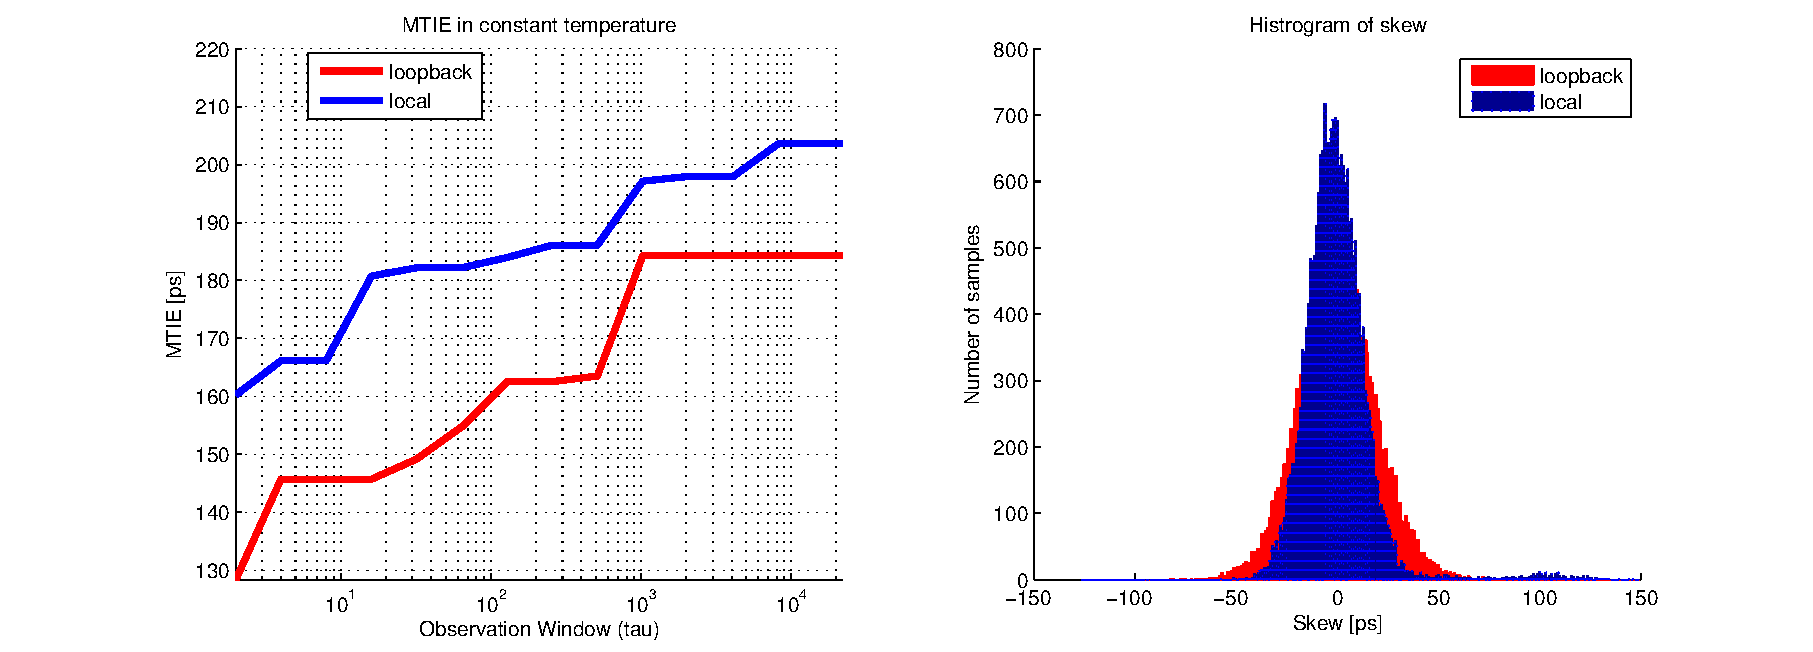
\includegraphics[width=0.5\textwidth]{../../figures/measurements/cngs_reference.eps}
\caption{\textbf{TEST 1}: parameters of the system in constant temperature (20 degrees Celsius).}
\label{fig:chamber-ref}
\end{figure}
% 

Firstly, the performance of the system was evaluated in a temperature-stabilized conditions of 
20 degrees Celsius. The measured 
system parameters are depicted in the column \textbf{TEST~1} of Table~\ref{tab:dataCompare} and in 
\figurename~\ref{fig:chamber-ref}.


\begin{figure}[!t]
\centering
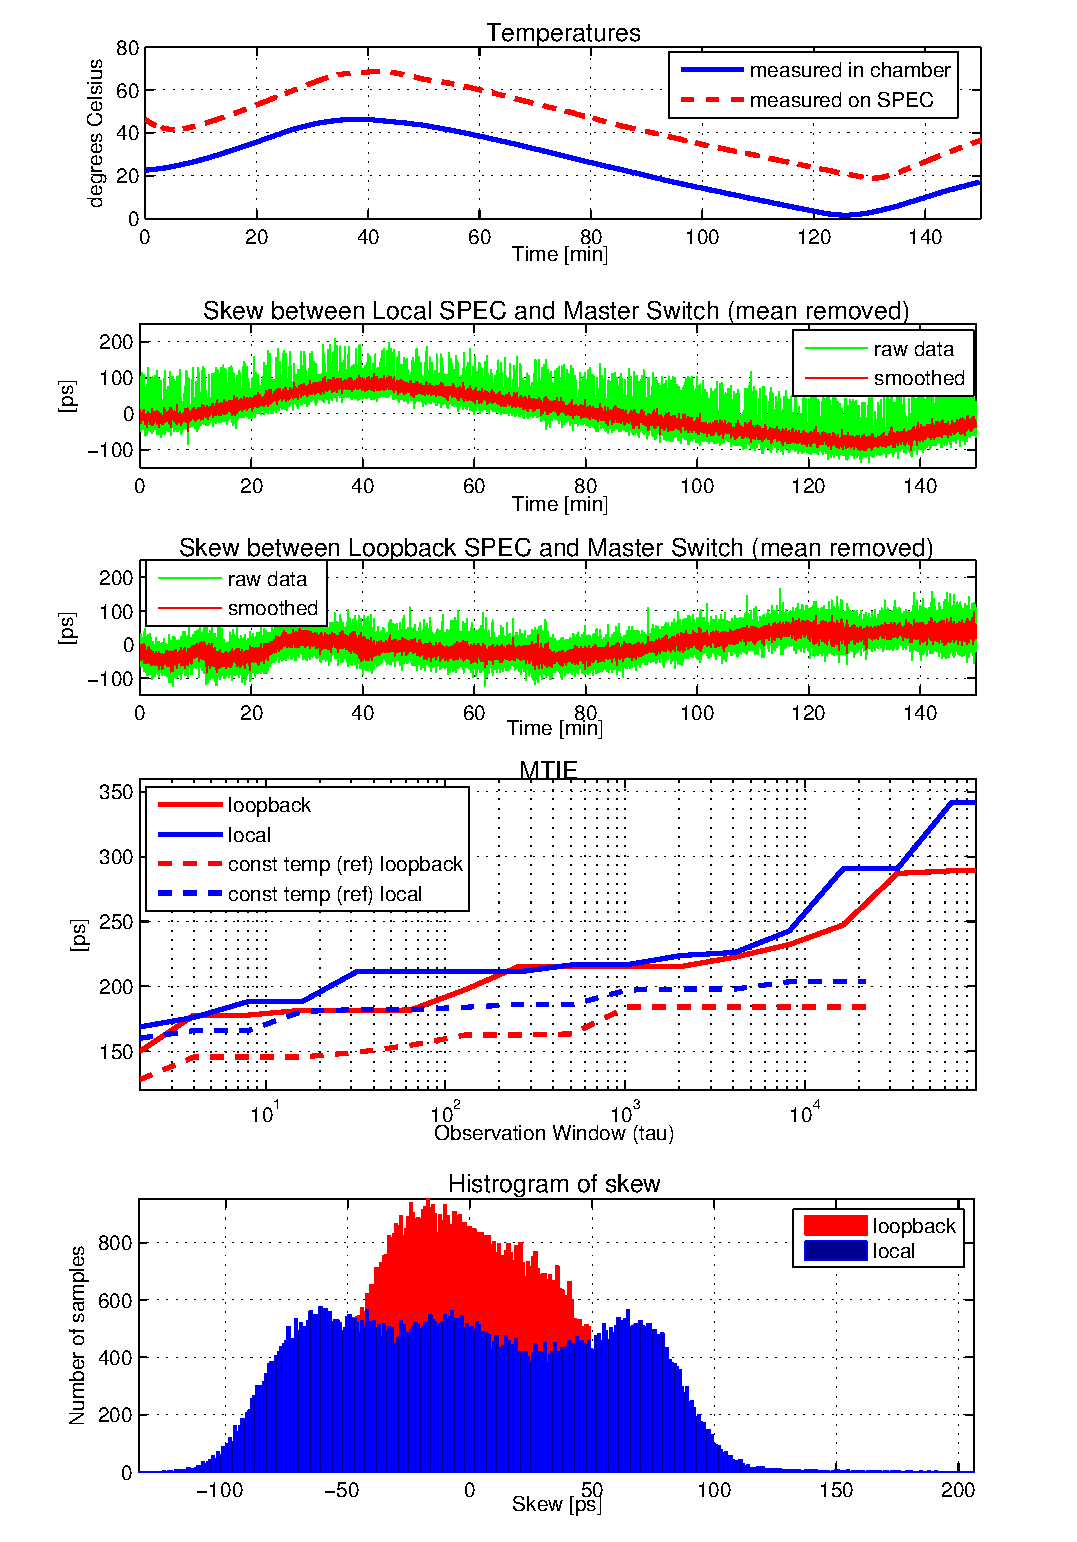
\includegraphics[width=0.5\textwidth]{../../figures/measurements/chamber-test.eps}
\caption{\textbf{TEST 2:} system performance when changing temperature of both SPECs.}
\label{fig:chamber-test}
\end{figure}


Secondly, both SPECs were placed in the climatic chamber while the rest of the setup
(i.e. two switches and fibers) were kept in the ambient temperature of the laboratory
(26$\pm$1.5~degrees Celsius). The test consisted of a single temperature cycle (described in
Section \ref{sec:tempTestSetup}) of 145 minutes. The measured system parameters are depicted in the 
column \textbf{TEST 2} of Table~\ref{tab:dataCompare} and in \figurename~\ref{fig:chamber-test}. 
The chamber's temperature (blue in the upper plot of
\figurename~\ref{fig:chamber-test}) as well as the SPEC's temperature (red) changed peak-to-peak
45 degrees Celsius. A fluctuation of the skew measured on the \textit{local} SPEC, depicted in the 
second plot in \figurename~\ref{fig:chamber-test},
is directly correlated with the temperature variation. This is due to the fact that the values of 
fixed delays (introduced by tx/rx hardware) compensated by the WRPTP protocol are assumed 
to be constant. This assumption holds for small temperature variation but introduces additional 
inaccuracy of synchronization over large temperature changes.
%, especially for short fibers. 
The skew of the \textit{loopback} SPEC (\figurename~\ref{fig:chamber-test}) is not directly 
correlated with the temperature.
However, it should be pointed out that the skew is measured between the \textit{loopback} SPEC and the 
grandmaster switch connected through another switch and a total of over 16~km of fiber. Therefore, what is 
observed in the plot is an addition of 
the temperature-induced fluctuation and a jitter introduced by the system (not related with 
temperature). \attention{Importantly}, the degradation
of the synchronization performance (depicted in MTIE plot in \figurename~\ref{fig:chamber-test}) 
over a considerable range of temperatures is reasonably small and does not prevent
the system from providing a sub-nanosecond synchronization accuracy and precision in the order of tens 
of picoseconds. 

Moreover, the clearly linear dependency between the variation of the temperature and that of the 
hardware delays can be easily compensated e.g. by providing a model of delays changes 
and applying their different values based on the temperature measurement from the SPEC's (or switch's) 
thermometer.


\begin{table}[!t]
\caption{Measured parameters of WR system during temperature tests}
\centering
\begin{tabular}{| l | c| c | c | c |c|}          \hline
                        &\textbf{TEST 1} & \textbf{TEST 2} \\   \hline
\textit{local} SPEC skew sdev [ps]    & 17             & 55              \\   \hline
\textit{loopback} SPEC skew sdev [ps] & 19             & 36              \\   \hline
\textit{local} SPEC MTIE         [ps] & $\leq$203            & $\leq$342             \\   \hline
\textit{looback} SPEC MTIE       [ps] & $\leq$184            & $\leq$289             \\   \hline
\end{tabular}
\label{tab:dataCompare}
\end{table} 

% 
% In the first test (TEST1) the performance of WR-timebase is evaluated in temperature-stabilized
% conditions with constant temperature of 20 degrees Celsius. The results are depicted in 
% \figurename~\ref{fig:chamber-ref} and included in Table~\ref{tab:dataCompare}.
% The performance of the WR-timebase in varying conditions is compared to the results in TEST 1. 
% 
% 

% \figurename~\ref{fig:chamber-test7} depicts results of the TEST 2 where the temperature of 
% the three fibers (10km, 5km and 10m) was changed over the time of 120 minutes. 
% It can be seen that the changes of the delay introduced by varying temperature are greatly 
% compensated. The skew of the local SPEC 
% is comparable with the one in the constant temperature (TEST 1). The skew of the loopback SPEC 
% increases in the order of 90ps (Table~\ref{tab:dataCompare}). The distribution of the loopback 
% skew is spread because of the addition of jitter introduced by both fibers (10km and 5km) 
% between the loopback SPEC and the grandmaster switch.
% 
% % \begin{figure}[!t]
% % \centering
% % \includegraphics[width=0.5\textwidth]{newFig/chamber-test7}
% % \caption{Climatic chamber test: changing temperature of fibers}
% % \label{fig:chamber-test7}
% % \end{figure}
% 
% 
% Variation of the temperature of the both SPECs in TEST 3 (\figurename~\ref{fig:chamber-test8}) 
% causes greater influence of the WR-timebase performance. The plot depicting the skew of 
% the local SPEC (\figurename~\ref{fig:chamber-test8}) clearly shows that the change of the
% hardware tx/rx elements of the SPEC causes skew fluctuation. The plot showing cable round trip 
% measurement explains what happens: the changes of the hardware delays (not compensated for) 
% causes virtual changes of the delay introduced by fiber, thus the non-existant change of 
% fiber temperature is compensated introducing decrease of synchronization precision. It is 
% worth noting that this effect is reasonably small for the tested range of temperatures (0-50
% degrees Celsius) and the MTIE is increased by less then 150 ps (Table~\ref{tab:dataCompare}).
% 
% Similarly, in TEST 4 the two switches were put into varying temperature conditions. The temperature
% variation of switches has substantially smaller effect on the performance of the local SPEC while
% substantially affects performance of the loopback SPEC. Still, the synchronization accuracy is 
% well within 1 ns. 
% 
% The last test, TEST 5, in which all the components of the system were put into varying conditions
% causes the comparable deterioration of the synchronization performance of the 
% WR-timebase. 



% \begin{table}[!t]
% \caption{Parameters comparison for different chamber test}
% \centering
% \begin{tabular}{| l | c| c | c | c |c|}          \hline
% TEST                    & \textbf{1} & \textbf{2} & \textbf{3} & \textbf{4}   & \textbf{5}\\   \hline
% local    skew sdev [ps] & 18         & 16         & 55         & 27           & 66 \\   \hline
% loopback skew sdev [ps] & 19         & 35         & 36         & 70           & 32 \\   \hline
% local MTIE         [ps] & 203        & 216        & 342        & 248          & 402 \\   \hline
% looback MTIE       [ps] & 184        & 275        & 289        & 442          & 322 \\   \hline
% \end{tabular}
% \label{tab:dataCompare}
% \end{table}

% All of the above tests show that the temperature variation of the WR system components has 
% direct effect on the synchronization performance of the system. However, the tests prove that
% the sub-nanosecond synchronization accuracy of the WR-provided timebase is guaranteed regardless
% of the temperature changes. 

